% Generado desde docs/INFORME.md. Editar libremente.

\section{5. API Gateway, políticas y fronteras de confianza}

Esta sección responde cómo se impide que alguien llegue a los servicios sin pasar por los controles. El API Gateway es la única puerta; el UML muestra sus piezas, las fronteras de confianza explican qué se revisa cada vez que una petición cruza de una zona a otra (del navegador al gateway, del gateway a un servicio, de un servicio a Vault) y al final se siguen dos solicitudes concretas, una autorizada y una denegada.


\subsection{UML del gateway y sus políticas}

\begin{figure}[H]
\centering
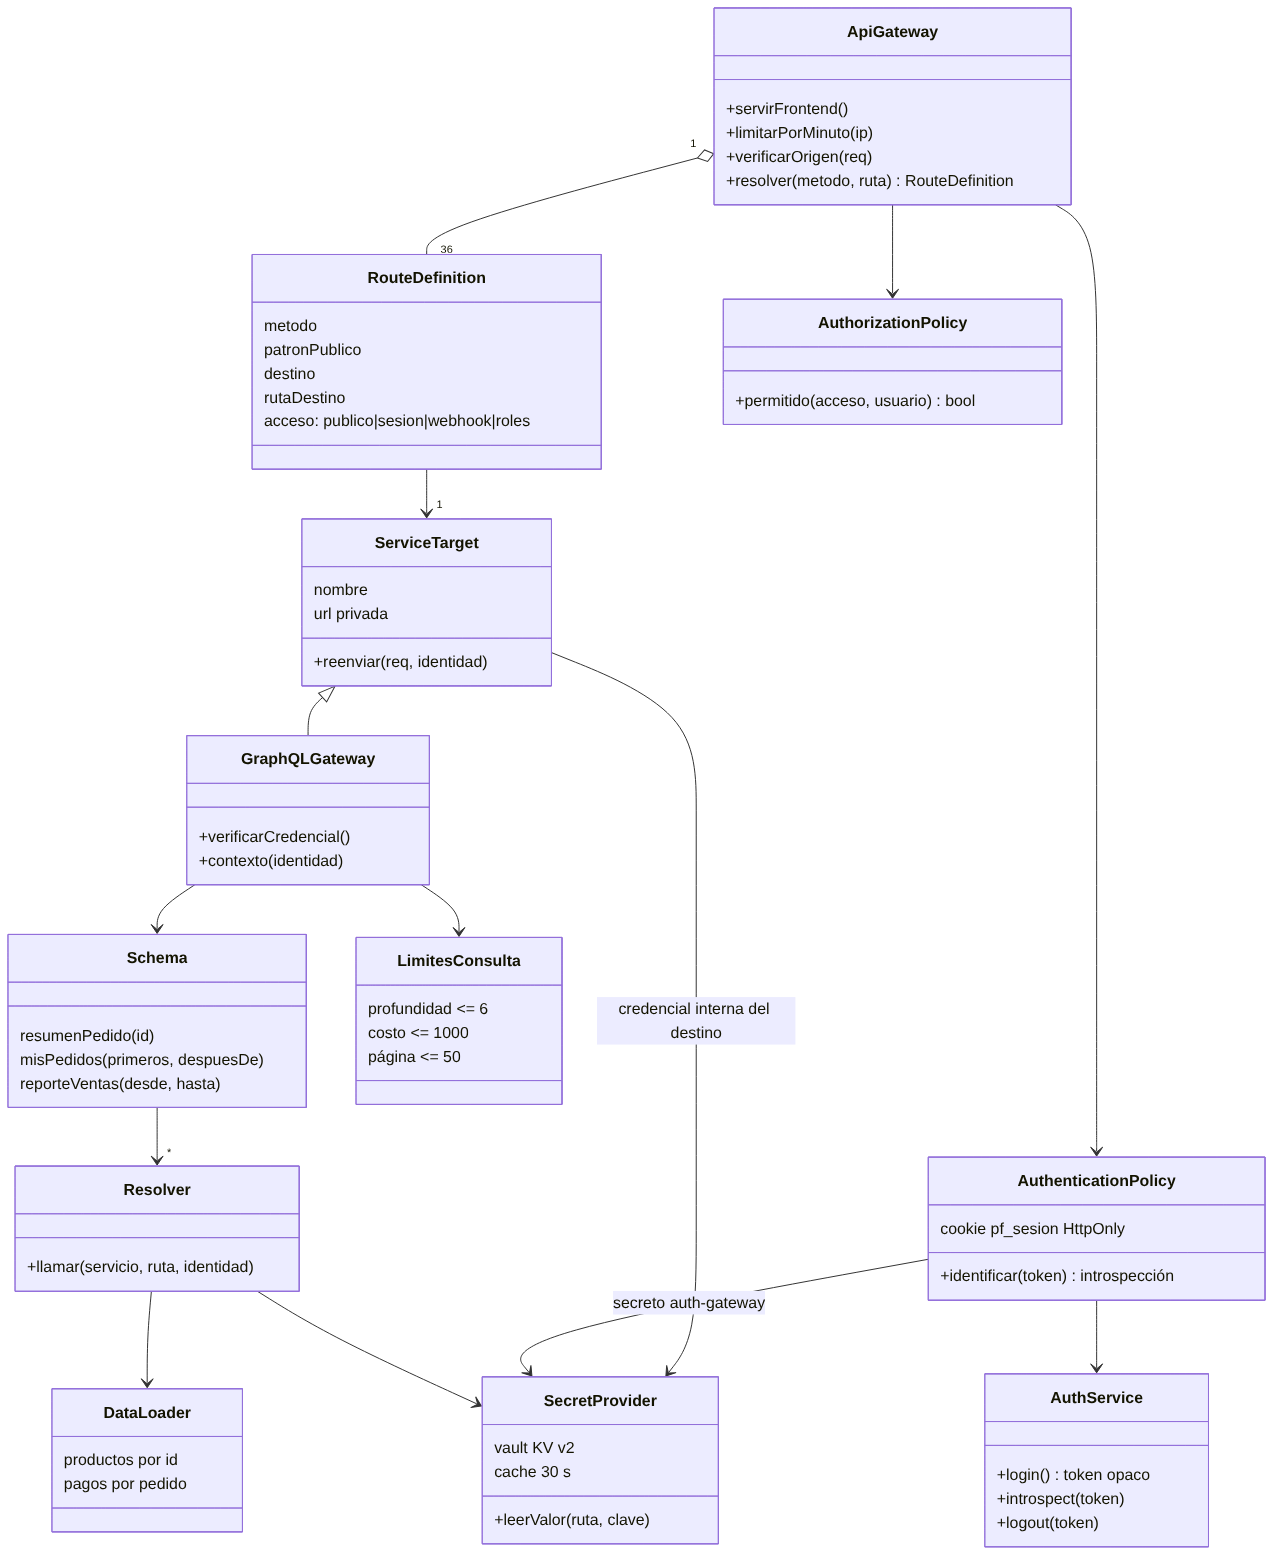
\includegraphics[width=\linewidth,height=0.85\textheight,keepaspectratio]{../diagramas/gateway.png}
\caption{UML del gateway}
\end{figure}

\begin{itemize}[nosep,leftmargin=*]
\item \textbf{RouteDefinition} (\texttt{gateway/\allowbreak{}src/\allowbreak{}rutas.\allowbreak{}js}): 36 filas; lo que no está, responde 404. Las rutas \texttt{/\allowbreak{}internos/\allowbreak{}*} de los servicios nunca se publican.
\item \textbf{AuthenticationPolicy} (\texttt{sesion.\allowbreak{}js}): cookie \texttt{pf\_\allowbreak{}sesion} HttpOnly; introspección en el Auth Service en cada petición.
\item \textbf{AuthorizationPolicy} (\texttt{rutas.\allowbreak{}js:\allowbreak{} permitido}): público, sesión, webhook o lista de roles.
\item \textbf{ServiceTarget} (\texttt{reenvio.\allowbreak{}js}): arma cabeceras nuevas, agrega la credencial del destino y la identidad, reenvía el cuerpo exacto; 502 si no responde, 504 si tarda más de 8~s.
\item \textbf{SecretProvider} (\texttt{vault.\allowbreak{}js}): lee de Vault con el token del gateway, guarda 30~s.
\item \textbf{GraphQLGateway, Schema, Resolver, DataLoader, LimitesConsulta}: en \texttt{graphql-\allowbreak{}gateway/\allowbreak{}} (sección 8).
\item No hay clientes gRPC (ADR 0001).
\end{itemize}

\subsection{Cuántos gateways y por qué}

Hay \textbf{un API Gateway externo} (puerto 8080) y, detrás de él, el \textbf{GraphQL Gateway privado}. No hay un segundo gateway público. Las políticas distintas (anónimo, cliente, personal, webhook) se separan con la columna de acceso de la matriz de rutas, que es lo que pide un solo gateway para separar rutas mediante políticas. Un segundo gateway, por ejemplo solo para el panel administrativo, duplicaría el contenedor, la superficie de ataque y las copias de CSRF, límites y sesión, sin una necesidad concreta: con 44 operaciones y un solo equipo, la ganancia sería nula. El GraphQL Gateway no es un segundo gateway público: es un servicio de agregación sin puerto publicado que hereda la sesión del primero (sección 8).


\subsection{Clasificación de rutas}

{\small
\setlength{\tabcolsep}{3pt}\renewcommand{\arraystretch}{1.15}
\begin{longtable}{|>{\raggedright\arraybackslash}p{\dimexpr 0.2140\linewidth-2\tabcolsep\relax}|>{\raggedright\arraybackslash}p{\dimexpr 0.3930\linewidth-2\tabcolsep\relax}|>{\raggedright\arraybackslash}p{\dimexpr 0.3930\linewidth-2\tabcolsep\relax}|}
\hline
\textbf{Clase} & \textbf{Operaciones} & \textbf{Observación} \\ \hline
\endfirsthead
\hline
\textbf{Clase} & \textbf{Operaciones} & \textbf{Observación} \\ \hline
\endhead
Externas anónimas & 12: S01, S02, S03, S07, S29, S33, S34, S35, S36, S38, S39, S44 & Una ruta pública de red no implica datos públicos: S35 devuelve la sesión si existe y S29 solo acepta una firma válida \\ \hline
Externas autenticadas & 18: S08, S09, S15, S16, S17, S18, S19, S20, S21, S22, S23, S24, S25, S27, S28, S30, S31, S37 & Pueden transportar datos restringidos para un usuario autorizado (sus pedidos, su ficha) \\ \hline
Administrativas (admin o dueño) & 14: S04, S05, S06, S10, S11, S12, S13, S14, S26, S32, S40, S41, S42, S43 & Mantenedores y reportes \\ \hline
Internas (nunca publicadas) & 11 & Inventario: cotizar, reservar y liberar. Clientes: ficha por id. Pedidos: confirmar pago. Pagos: devoluciones y pagos por pedido. Auth: introspección, crear cuenta, cambiar cuenta de un cliente y estado de verificación \\ \hline
\end{longtable}
}

\subsection{Fronteras de confianza}

\begin{figure}[H]
\centering
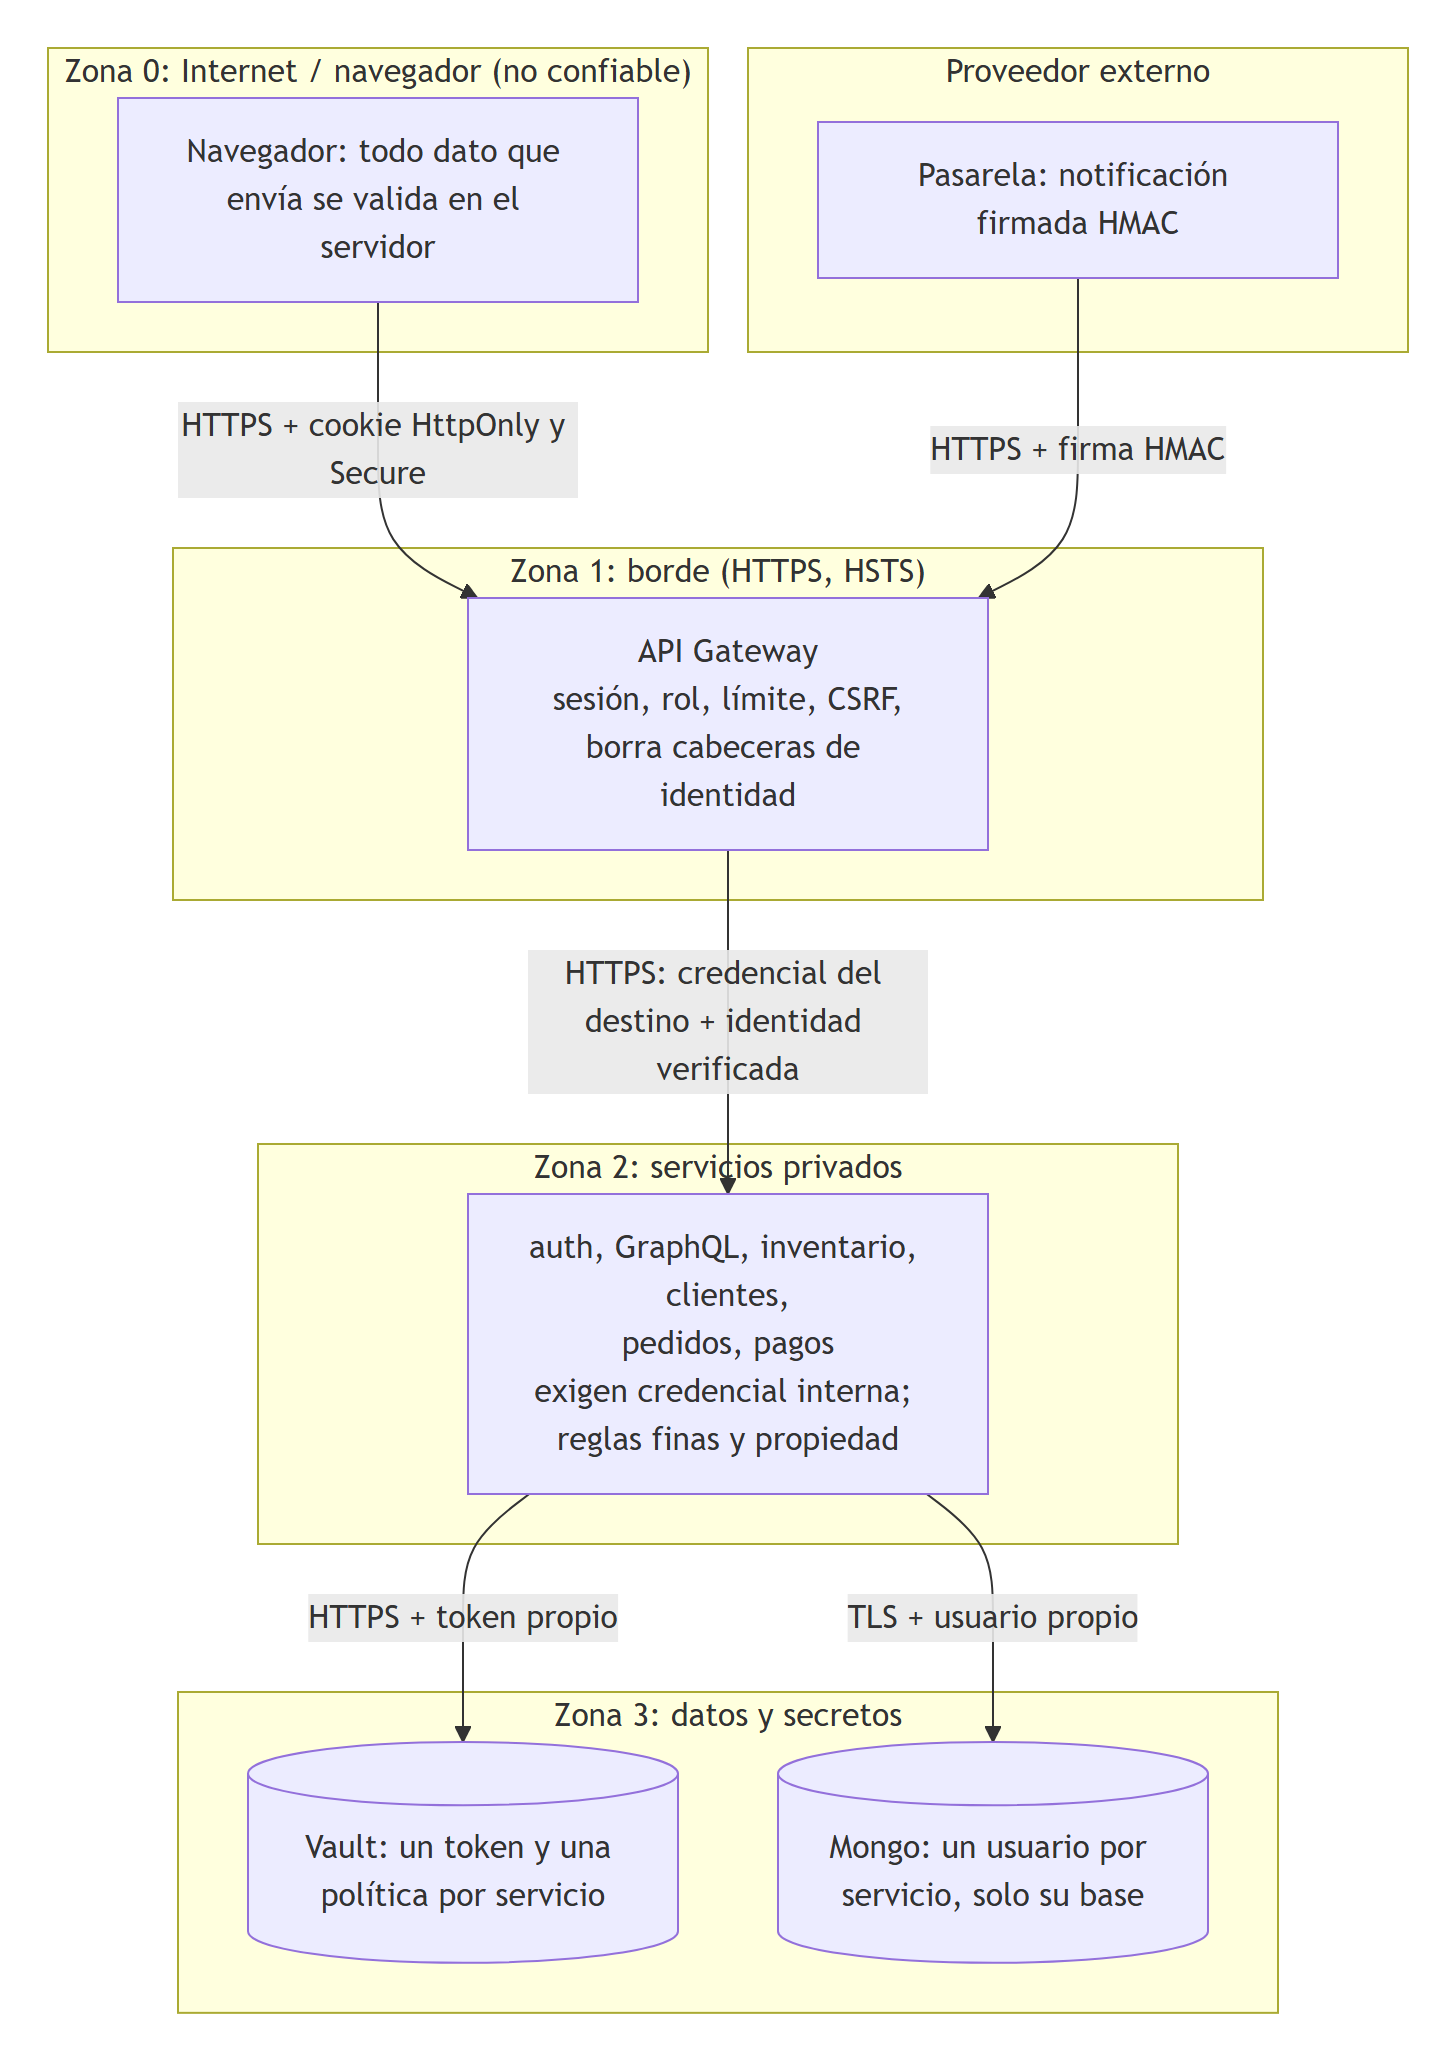
\includegraphics[width=\linewidth,height=0.85\textheight,keepaspectratio]{../diagramas/fronteras.png}
\caption{Fronteras de confianza}
\end{figure}

{\small
\setlength{\tabcolsep}{3pt}\renewcommand{\arraystretch}{1.15}
\begin{longtable}{|>{\raggedright\arraybackslash}p{\dimexpr 0.3149\linewidth-2\tabcolsep\relax}|>{\raggedright\arraybackslash}p{\dimexpr 0.6851\linewidth-2\tabcolsep\relax}|}
\hline
\textbf{Frontera} & \textbf{Qué se verifica al cruzarla} \\ \hline
\endfirsthead
\hline
\textbf{Frontera} & \textbf{Qué se verifica al cruzarla} \\ \hline
\endhead
Navegador $\rightarrow$ gateway & TLS (HTTPS con HSTS), sesión (cookie + introspección), rol, origen (CSRF), límite por IP, tamaño del cuerpo (100~KB). Se descartan \texttt{X-\allowbreak{}Usuario-\allowbreak{}*}, \texttt{X-\allowbreak{}Credencial-\allowbreak{}Interna}, \texttt{Authorization} y la cookie antes de reenviar \\ \hline
Pasarela $\rightarrow$ gateway $\rightarrow$ pagos & Firma HMAC del cuerpo exacto, token y monto \\ \hline
Gateway $\rightarrow$ servicio & Credencial interna del servicio de destino (cada servicio tiene la suya) \\ \hline
Servicio $\rightarrow$ servicio & Credencial del destino + identidad del usuario original (el destino aplica sus reglas) \\ \hline
Servicio $\rightarrow$ Vault & Token propio con política de solo lectura en sus rutas \\ \hline
Servicio $\rightarrow$ Mongo & Usuario propio con \texttt{readWrite} solo en su base, sobre TLS \\ \hline
Todos los saltos & TLS 1.2 o superior: el cliente verifica el certificado del servidor con la CA de prueba (en Node, \texttt{NODE\_\allowbreak{}EXTRA\_\allowbreak{}CA\_\allowbreak{}CERTS}; en Python, \texttt{SSL\_\allowbreak{}CERT\_\allowbreak{}FILE}; en Mongo, \texttt{tlsCAFile}). Un intento en claro contra un servicio interno se rechaza (caso 7.12 y comprobación manual) \\ \hline
\end{longtable}
}

\subsection{Decisiones de separación}

\begin{itemize}[nosep,leftmargin=*]
\item El frontend se sirve desde el gateway: misma origen que la API, la cookie viaja sin CORS y puede ser \texttt{SameSite}.
\item El gateway no tiene reglas de negocio: solo el control grueso. La propiedad del recurso la decide el servicio dueño (así no se puede saltar llamando por GraphQL).
\item El GraphQL Gateway está detrás del API Gateway, no al lado: hereda sesión, límites y CSRF.
\item Pagos es el único servicio privado en la red \texttt{externa}, porque es el único que habla con el proveedor.
\end{itemize}

\subsection{Recorrido de una petición autorizada y una denegada}

\begin{figure}[H]
\centering
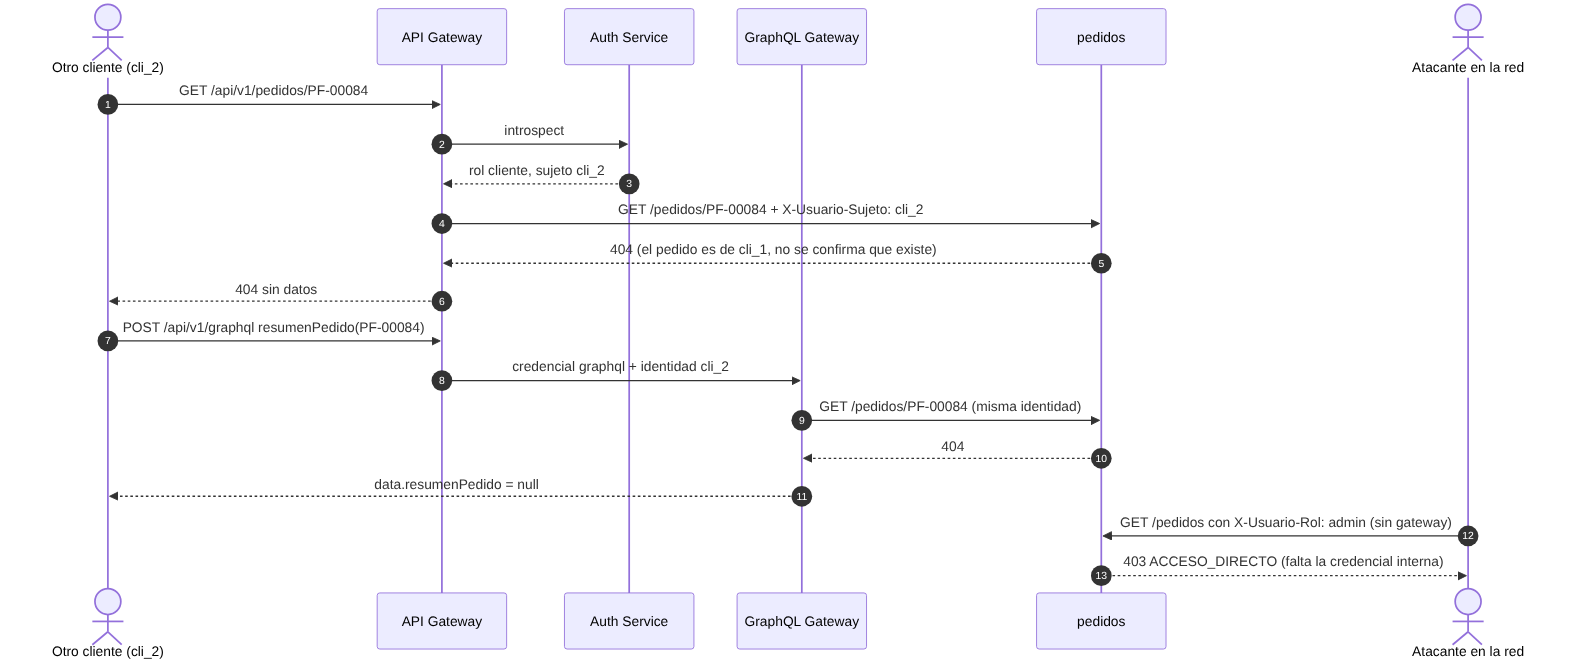
\includegraphics[width=\linewidth,height=0.85\textheight,keepaspectratio]{../diagramas/secuencia-denegada.png}
\caption{Secuencia denegada}
\end{figure}

\textbf{Autorizada:} la cocina acepta el pedido PF-00084. Navegador $\rightarrow$ \texttt{POST /\allowbreak{}api/\allowbreak{}v1/\allowbreak{}pedidos/\allowbreak{}PF-\allowbreak{}00084/\allowbreak{}aceptar} con su cookie $\rightarrow$ el gateway introspecciona (rol \texttt{cocina}) $\rightarrow$ la matriz permite \texttt{admin,\allowbreak{} cocina} $\rightarrow$ lee de Vault la credencial de pedidos $\rightarrow$ reenvía con \texttt{X-\allowbreak{}Usuario-\allowbreak{}Rol:\allowbreak{} cocina} $\rightarrow$ pedidos verifica la credencial, que el rol sea cocina o admin, que el pedido esté PAGADO (en el mismo \texttt{update}) y registra el paso con el nombre de quien lo hizo $\rightarrow$ \texttt{200}. Evidencia: caso 10.4.


\textbf{Denegada:} otro cliente pide el mismo pedido. El gateway lo deja pasar (los clientes pueden ver pedidos), pero pedidos compara \texttt{X-\allowbreak{}Usuario-\allowbreak{}Sujeto} con el dueño y responde 404, sin confirmar que existe. Por GraphQL ocurre lo mismo, porque el GraphQL Gateway reenvía la identidad. Si alguien en la red privada llama directo a pedidos con \texttt{X-\allowbreak{}Usuario-\allowbreak{}Rol:\allowbreak{} admin}, recibe 403 por no tener la credencial interna. Evidencia: casos 7.5 y 7.9.

